\section{MUSIC-algoritmin simulointi}
Tässä kandidaattityössä käytettiin Matlab-ohjelmaa simuloimaan MUSIC-algoritmia ja sen eri versioita. Simulaatioita tehtiin yksinkertaisella pallomallilla sekä todellisten aivojen mallilla, jotka muodostettiin MRI-kuvantamisen avulla.

MUSIC-algoritmia voidaan testata yksinkertaisella pallomallilla. Tässä mallissa elektrodit ja lähdepisteet sijotetaan pallokuoren yläpäähän ja sitten projisoidaan stereograafisen projektion avulla tasoon.



\clearpage
\begin{figure}[h]
    \centering
    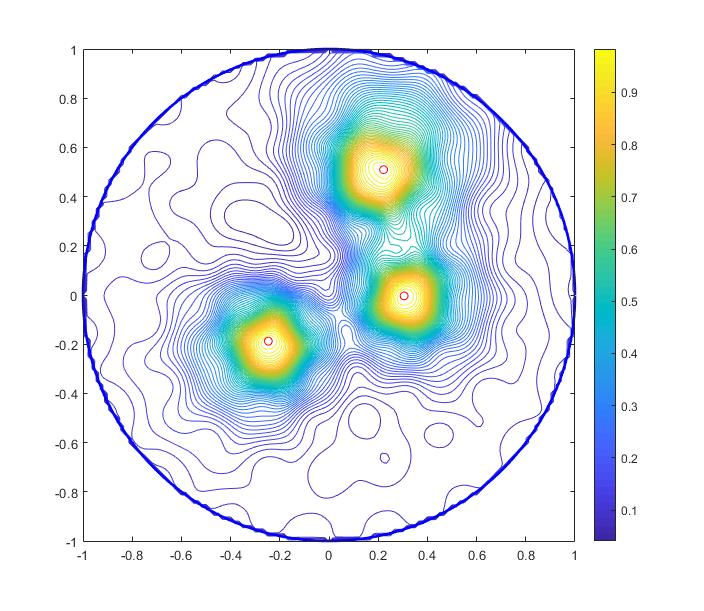
\includegraphics[scale=0.38]{mfix.jpg}
    \caption{MUSIC-algoritmin simulointi pallomallilla kiinnitetyllä orientaatiolla.}
    \label{fig:mfix}
\end{figure}

\begin{figure}[h]
    \centering
    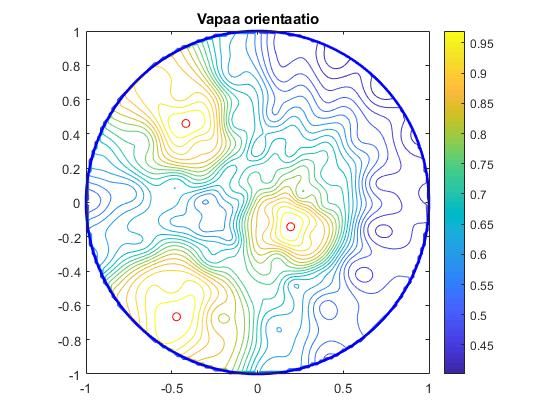
\includegraphics[scale=0.4]{mfree.jpg}
    \caption{MUSIC-algoritmin simulointi pallomallilla vapaalla orientaatiolla.}
    \label{fig:mfree}
\end{figure}

Kuvista huomataan, että MUSIC vapaalla orientaatiolla saa aikaan suuria aktiivisuuden alueita, mikä vaikeuttaa lähteiden paikantamista.

\begin{figure}[h]
    \centering
    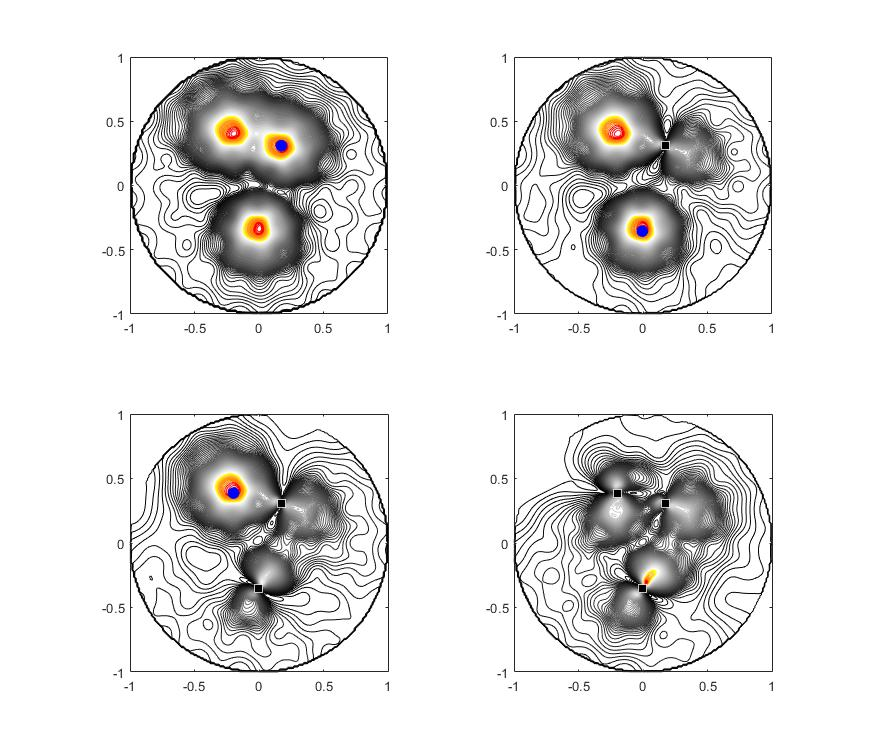
\includegraphics[width=1\textwidth]{rap11.jpg}
    \caption{RAP-MUSICin testausta pallomallilla ja kolmella lähteellä. Punainen väri kuvaa aktiivista aluetta. Algoritmin löytämä lähde on merkitty sinisellä ympyrällä ja löydetyt lähteet valkoreunaisella neliöllä}
    \label{fig:RAP}
\end{figure}

